
\documentclass{eieproyecto}
\usepackage{hyperref}
\usepackage{xcolor}
\hypersetup{
 colorlinks=false,
 pdfborder={0 0 0},
}
\usepackage{graphicx}
\usepackage{subcaption}
\usepackage{wrapfig}
\usepackage{amsmath,amssymb}
\DeclareMathOperator{\E}{\mathbb{E}}
\usepackage[linesnumbered,ruled]{algorithm2e}
\usepackage{wasysym}

\begin{document}
\frontmatter

\title{Sistemas de trading y Deep Reinforcement Learning}

\autor{Leonardo Jose Caramello}

%fecha de la presentación oral
\date{Agosto - 2017}

%tribunal evaluador
%profesor guía
\dca{Diego Martinez}
 
 
\eietitlepage 
\cleardoublepage 
\eieaprovalpage 
\clearpage

%Archivo con el texto del resumen
% este no debe exceder una página
\begin{center}\huge{\textbf{Resumen}}\end{center}

%--------------------------------------------------------------------
\noindent
\\
\\
Vivimos en un mundo cada vez más digitalizado donde el acceso a la información es cada vez más fácil y abundante, un mundo que en los últimos años se ha transformado radicalmente y que sin duda lo seguirá haciendo en los años venideros. Los avances en machine learning, han permitido automatizar tareas, que hasta hace algunos años parecía imposible, en la actualidad podemos encontrar múltiples ejemplos de ellos, como por ejemplo, waymo(Google self-driving car), los sistemas de recomendación como los usados por netflix o mercado libre, o Deep Mind.
\\
\\
Uno de los desafíos más interesantes en este área, es el desarrollo de sistemas de trading que permitan automatizar la comercialización de activos financieros, con el fin de administrar eficientemente un porfolio de inversiones.
El siguiente trabajo esta inspirado en Deep Mind \cite{8}, un agente que combinando reinforcement learning y deep learning aprende a jugar juegos de Atari. \\
En este paper buscaremos investigar la aplicabilidad y efectividad de las técnicas utilizadas en deep mind, en el desarrollo de sistemas de trading. 



\clearpage

\listoffigures 
%Lista de la nomenclatura utilizada en el texto
% constantes, variables, símbolos, acrónimos, etc.

\chapter{Nomenclatura}
%--------------------------------------------------------------------

\begin{description}[labelindent=1cm,labelwidth=2.25cm,align=left,leftmargin=3.45cm]  %no cambiar esta línea
	\item[$s$] estado
	\item[$a$] acción
	\item[$t$] tiempo discreto
	\item[$T$] Instante final de la simulación o el episodio
	\item[$S$] Conjunto de estados
	\item[$A(s)$] conjunto de acciones validas en el estado s.
	\item[$S_t$] Estado en el que se encuentra el agente en el instante t.
	\item[$A_t$] Acción elegida por el agente en el instante t.
	\item[$R_t$] Reward obtenido por el agente en el instante t+1
	\item[$\pi$] política de decisión, regla de decisión.
	\item[$\pi(s)$] acción tomada en el estado s, siguiendo la política determinista $\pi$ 
	\item[$q_\pi(s, a)$] el valor de tomar la acción a, en el estado s, bajo la política de decisión $\pi$
	\item[$q_*(s, a)$] el valor de tomar la acción a, en el estado s, bajo la política de decisión $\pi$
	\item[$\gamma$] factor de descuento de rewards.
    \item[$\alpha$] razón de aprendizaje
    \item[$\varepsilon$] probabilidad de elegir una acción aleatoria en una política de decisión greedy
\end{description}

\clearpage

\mainmatter
\pagestyle{eieheadings}

\chapter{Introducción}

Este documento forma parte del proyecto final de carrera y se acompaña junto con el código del agente desarrollado, disponible también \href{https://github.com/jcaramello/deepQ-stock/}{\textcolor{blue}{online}}. En este documento se pretende dar una presentación formal a los resultados de investigación obtenidos durante el desarrollo del proyecto, como así también una descripción del problema a resolver y de la solución adoptada, detallando cuales fueron cada una de las decisiones de diseño tomadas y el por que de estas	.

\section{Alcance del proyecto}
El proyecto se planteo como un trabajo de investigación que permitiera analizar cuales son las herramientas que brinda el machine learning para desarrollar un agente capaz de invertir en activos financieros(acciones, bonos, obligaciones negociables, etc), en particular, a través  del uso de reinforcement learning.

El proyecto pretende ser una prueba de concepto, que permita abordar el desarrollo de sistemas de trading utilizando reinforcement learning. En particular, se buscara identificar cada uno de los componentes que plantea el framework de reinforcement learning, de forma tal, de tratar de encontrar una representación adecuada.
\\
A su vez, durante el proceso de investigación se tratara de comprender la complejidad y las problemáticas propias del dominio del problema, en este caso, los mercados financieros y el trading en ellos, las cuales sera necesario comprender, para poder modelar una solución mas eficiente.
\\
Queda fuera del alcance de este proyecto lo siguiente:

\begin{itemize} % lista con viñetas
	\item Desarrollar un explicación detallada del funcionamiento de reinforcement learning o de deep learning.
	\item Desarrollar un nuevo algoritmo de RL
	\item Desarrollar un agente capaz generar ganancias
	\item Desarrollar una comparación entre diferentes implementaciones y/o algoritmos del RL.
    \item Intentar cubrir todas las peculiaridades de un mercado financiero.
\end{itemize}

\section{Objetivos}
A continuación se detallan los objetivos del proyecto

\subsection{Objetivo general}
Investigar la posible aplicabilidad de reinforcement learning en el desarrollo de sistemas de trading que permitan optimizar y automatizar la toma de decisiones de un potencial inversor.

\subsection{Objetivos específicos}

\begin{itemize} % lista con viñetas
	
	\item Brindar una descripción general del funcionamiento de los mercados financieros.
	\item Brindar una descripción general de Reinforcement Learning.
	\item Brindar una especificación detallada de cómo modelar el problema de trading utilizando los elementos que propone el framework de RL.
	\item Desarrollar un entorno que permita realizar la simulación de un mercado financiero 
	\item Desarrollar un agente inteligente capaz de percibir su entorno y tomar decisiones de compra y/o venta de un activo financiero
\end{itemize}

\section{Metodología}
En primer lugar se definirá el tópico central de la investigación, junto con los alcances y limitaciones del proyecto.
En una segunda etapa, se hará una investigación sobre el funcionamiento de los mercados financieros, en particular, se buscará entender el funcionamiento del análisis técnico de los mercados  y/o de los principales indicadores bursátiles, de forma tal de poder capturar estos conceptos y poder modelarlos en el desarrollo del agente.  
En tercer lugar se llevará a cabo una investigación de los diferentes algoritmos de RL y de cómo modelar el problema de trading utilizando los elementos que propone el framework.
Por último, se proseguirá con el desarrollo del agente inteligente, de forma tal de poder integrar todo el conocimiento adquirido en las etapas previas. 

\section{Contenido}
Por último, concluimos este capitulo introductorio con una breve descripción de cada uno de los capítulos siguientes

\begin{itemize} % lista con viñetas
	\item Capitulo 2 - Mercados Financieros: En este capitulo se presenta el problema de trading, se dará una breve explicación del funcionamiento de un mercado financiero y de como operan los inversores en el, abarcado conceptos como acciones, precio, análisis técnico vs análisis fundamental, drivers, indicadores bursátiles, tendencias, etc.
	\item Capitulo 3 - Reinforcement learning y deep learning: En este capitulo se introducirá brevemente el framework de reinforcement learning y cada uno de sus componentes, para luego esbozar la representación que se adoptara junto con un pseudo algoritmo que mostrara una primera aproximación a la solución elegida
	\item Capitulo 4 - Arquitectura y Diseño: Aquí se hará una descripción detallada de la arquitectura y el diseño del sistema implementado, se mostraran detalles y demás peculiaridades de implementacion, en particular parámetros de configuración, funcionalidades, etc. Se mostraran algunas las partes mas relevantes del código del agente.
	\item Capitulo 5 - Evaluación y desempeño: En esta sección analizaremos el desempeño y eficacia de la solución implementada, mostrando y analizando los diferentes resultados obtenidos durante la ejecución del agente.
	\item Capitulo 6 - Conclusiones: Como punto final, esta sección estará destinada a comentar diferentes conclusiones que pudimos establecer, junto con algunas recomendaciones y/o observaciones de posibles mejoras a futuro.
	\item Capitulo 7 - Bibliografía: Listado de las diferentes referencias que formaron parte de la investigación.
\end{itemize}
\chapter{Mercados Financieros}

\section{Introducción}
En economía, un mercado financiero es un espacio (físico, virtual o ambos) en el que se realizan los intercambios de instrumentos financieros y se definen sus precios. Los mercados financieros están afectados por las fuerzas de oferta y demanda. La clave del éxito está en saber predecir el futuro y actuar en consecuencia. Quedarse largo en una posición (comprar) si se piensa que el mercado va a subir, o deshacer posiciones o quedarse corto si se piensa que el mercado va a bajar. Si se consigue hacer esto en forma reiterada se podrán obtener ganancias y con ello incrementar el capital inicial.

\section{Análisis Técnico y Análisis Fundamental}
Para intentar saber cómo va a estar un valor en el futuro, se distinguen tradicionalmente dos corrientes bien diferenciadas: los que siguen el análisis técnico y los que siguen el análisis fundamental. Los fundamentales se basan en que el valor de una acción esta dado por los beneficios futuros de la empresa. Ni más, ni menos. Lo que intentan es determinar cuáles serán esos beneficios futuros, y para ello tratan de conocer diferentes detalles de la empresa: noticias que les afecten, posibles movimientos societarios, estrategias, competidores, nuevos productos, etc. Toda la información micro económica tiene impacto en dichos beneficios futuros. Así como también la macro económica: cómo evoluciona el entorno general de la empresa, el entorno regulatorio, el entorno político, etc. Se trata, en definitiva, de analizar la mayor cantidad de información posible, y de convertir esa información en cuentas de resultados provisionales que se puedan descontar para hallar el valor actualizado de la acción. 
El análisis técnico, por el contrario, se basa en que el precio de la acción lo descuenta todo. Es decir, todos los factores relevantes a la inversión, cualquiera que ellos sean, pueden ser reducidos al nivel de precios de la acción y volumen transado. El precio de mercado representa el total conocimiento de los inversionistas respecto de cualquier activo dado en un momento particular. Además, refleja todas las noticias sobre el mercado así como la suma de conocimientos de los participantes en éste.  Aquí se habla de tendencias alcistas o bajistas, de líneas de soporte (cotizaciones donde se cree que la acción dejará de bajar y tendrá un "rebote"), líneas de resistencia (cotizaciones en las que el valor de la acción se atascará y que le costará "romper"), etc. 
La lógica nos dice que el análisis fundamental es el que tiene más sentido. Sin embargo, en la realidad esto no siempre es así. Lo cierto es que cuanta más gente crea en los análisis técnicos, más probabilidad tendrán de ser reales sus predicciones (ya que la gente actuará como si fueran reales, contribuyendo a su efectiva realización).
\\\\
Este proyecto se basa fundamentalmente en las ideas del análisis técnico y las herramientas que este brinda, las cuales, serán los pilares fundamentales sobre los que el agente tomara sus decisiones.
Para comprender un poco mas acerca de este y visualizar como es posible tomar decisiones acertadas solamente apoyándonos en el análisis técnico, debemos mirar mas en detalles, algunos aspecto de la teoría clásica financiera.

\section{Teoría Clásica}

Gran parte de la teoría financiera clásica parte del principio fundamental que los inversores son racionales y que los precios del mercado reflejan en todo momento y de manera instantánea el valor fundamental de los títulos.
Este principio fundamental establece que la competencia entre los distintos participantes que intervienen en el mismo, conduce a una situación de equilibrio en la que el precio de mercado de un activo constituye una buena estimación de su precio teórico, es decir, que los precios que se negocian en el mercado reflejan toda la información existente y se ajustan total y rápidamente a los nuevos datos que puedan surgir. La consecuencia de este principio es que un inversor racional no puede hacer nada para “ganar” al mercado.\\	

De acuerdo con este principio de racionalidad económica, lo que debe hacer un inversor es intentar maximizar su riqueza final. Para lograr esto, lo mejor que puede hacer este inversor racional es invertir en el mercado de manera diversificada de una forma igual a la del mercado y permanecer en esta misma cartera salvo por necesidades de liquidez o debido a variaciones de su situación actual o de cambio en sus necesidades futuras.
\\\\
A pesar de la cantidad de libros de texto y de artículos que sostienen los principios anteriores sobre la forma en que deben comportarse los inversores, lo cierto es que la evidencia empírica nos dice que las cosas no suceden de la forma en la que deberían suceder según este principio,o por lo menos, no enteramente.
Para poder explicar este fenómeno deberemos detenernos en algunos aspectos fundamentales en el proceso de decisión de los inversores. 
\\
Un claro ejemplo de esto podemos verlo si analizamos el proceso de decisión de venta, de acuerdo con la teoría clásica, los precios de cualquier activo siguen un movimiento aleatorio. Esto significa que la mejor predicción sobre el precio futuro es la que se tiene hoy. La consecuencia inmediata de esto es que no tiene ningún sentido vender, para a continuación, volver a comprar éste mismo activo u otro diferente.
Dado que las expectativa de ganancia debido a la diferencia entre los precios venta y de compra sería nula. Solo tendríamos una pequeña pérdida debido al coste de la transacción.
En otras palabras, el mercado no es predecible y, en consecuencia, no es posible obtener un beneficio realizando trading. Sin embargo, veamos algunos conceptos que contradice esto:

\begin{itemize}
	\item \emph{La creencia de los inversores en la reversión a la media}, es el principio según el cual existe un valor medio de cada acción al cual se acaba volviendo en algún momento. Así, si un valor tiene un precio que el inversor cree que está por debajo del que le corresponde (su valor “medio”) , tarde o temprano, el precio de esta acción subirá hasta llegar a ese precio. Y, en consecuencia, recuperará las pérdidas que está teniendo en este momento. Lo mismo puede decirse cuando el valor esta por encima del valor medio. Así, si el inversor tiene una serie de valores que entiende que están infravalorados por el mercado, tiende a mantenerlos esperando que vuelvan a su valor “medio”.  	

	\item \emph{La aversión a la pérdida. } Si por alguna razón, tenemos alguna predicción confiable que nos dice que el precio de un activo va a bajar, lo racional es vender, independientemente de que con el activo a vender se obtenga un beneficio por su venta o no.
	La realidad nos muestra que esto no siempre es así, y que en general, los inversores tienden a no realizar las pérdidas, es decir, a no efectuar la venta real, en valores en los que pierden y, en cambio, vender antes de tiempo aquellos en lo que tienen ganancias. Una gran parte de los inversores venden valores ganadores y mantienen los perdedores.
	
	\item \emph{El efecto disposición}. El comportamiento debido a la aversión a la pérdida es una parte de un comportamiento más general de los inversores, llamado efecto disposición según el cual, los inversores mantendrían demasiado tiempo activos en pérdidas y venderían demasiado pronto activos con ganancias. Esto se da debido a que los inversores son mucho más sensibles a las pérdidas que a las ganancias en el sentido de que las primeras influyen el doble que las segundas.
	
	\item \emph{El efecto atención}. Los inversores tienden a invertir en aquellos valores que llaman mas su atención por la razón que sea, incluso aunque esta atención sea debida a noticias negativas, y como consecuencia, gran parte de los inversores diversifica mucho menos de lo que debería.
\end{itemize}

Estos argumentos y otros, nos indican que el inversor no siempre se comporta de manera esperada. Tal vez, el principal error de la teoría clásica sea partir de que los inversores son entes racionales y que no operan según sentimientos, euforia, miedo, avaricia o codicia.

\section{Fundamentos del análisis técnico}

Si bien es cierto que existen diversos argumentos en contra del análisis técnico, como por ejemplo:

\begin{itemize}
	\item La profecía del auto cumplimiento
	\item El pasado no sirve para predecir el futuro
	\item El paseo aleatorio
	\item Mercados Eficientes
\end{itemize}

Lo interesante aquí es entender que el análisis técnico no trata de predecir el valor futuro del precio de un activo, sino mas bien de responder la siguiente pregunta:\\\\

\emph{¿cómo cree el conjunto de inversionistas que evolucionará el precio en el futuro? }
\\

Es importante notar, que lo que importa no es la evolución del precio, sino lo cree \emph{la masa de inversores sobre la evolución del precio}, y ¿Por que esta pregunta es relevante?. Pues por que en el corto y mediano plazo, los precios se mueven mas por cuestiones psicológicas de los inversores que por variables financieras.\\

El análisis técnico nos dará las herramientas necesarias poder analizar desde un punto de vista estadístico y probabilisto, cual fue el comportamiento de la masa de inversores en el pasado, ante una situación similar, para luego poder tomar la decisión mas conveniente.
\\\\
En otras palabras lo que se busca es reducir el nivel de incertidumbre que tiene el inversor a la hora de decidir si compra o vende un activo, haciendo uso de diferentes herramientas matemáticas como las medias móviles, lineas de tendencias o patrones con el objetivo de determinar cual es el comportamiento mas probable de la masa de inversores.



\chapter{Reinforcement Learning y Deep Learning}


\section{Introducción}

En esta sección buscaremos dar una descripción mas detallada, tanto del problema a resolver, como así también de como se aplicaron los conceptos de reinforcement learning y deep learning a las soluciones adoptas durante el desarrollo del mismo. Esta sección no pretende ser una guía o una introducción a reinforcement learning, ni a deep learning, sin embargo es necesario contar con conocimientos básicos de ellos para poder comprender los detalles de la solución propuesta. Dejamos en manos del lector la capacitación en estos a través de los diferentes recursos que pueden hallarse en linea. (ver Capitulo 7 - Bibliografía).
\\\\
Recordemos que el objetivo es desarrollar un agente inteligente, que a partir de un capital inicial, sea capaz de realizar compras y ventas de un activo financiero. El agente no poseerá ningún conocimiento previo acerca del funcionamiento del mercado, ni de la empresa sobre la que opera, ni ningún otro tipo de información. Solo conocerá el precio actual de la acción, y su evolución durante los días previos, junto un conjunto de indicadores bursátiles. 
\\
El agente va a interactuar con un simulador de un mercado bursátil, esta interacción se llevará a cabo siguiendo una serie de acciones, observaciones y recompensas.
Cada interacción será llevada a cabo en episodios que tendrán una duración de m días
\\

\begin{figure}[h!]
	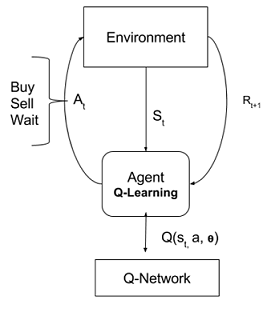
\includegraphics[scale=0.5]{imagenes/deepRLOverview.png}
	\caption{Reinforcement Learning Architecture Overview.}
\end{figure}


En cada instante t, el agente tendrá que seleccionar una acción $a_t$  de un conjunto válido de acciones A = {$a_1, a_2, …, a_n$}. La acción será pasada al entorno, el cual modificará su estado interno y como respuesta a esta interacción el agente recibirá una recompensa $R_{t + 1}$, la cual será calculada por el entorno. El entorno será estocástico, es decir, su comportamiento será no determinístico. Cada uno de los estados contendrá información relevante sobre el papel, como el precio, el volumen, y diferentes indicadores bursátiles, como medias móviles, medias móviles exponenciales, etc.

\section{Configuración de estados}

Ya sea de que se trate de un inversor experimentado o un agente inteligente, difícilmente sea posible tomar una decisión acertada sobre, la compra o venta de un activo, solamente mirando lo que sucede con el precio actual 
del activo, es necesario considerar una ventana de tiempo de tamaño n, para poder analizar la variación que ha tenido y así poder determinar la situación actual del activo, es decir, si se encuentra en una tendencia
alcista o bajista, si se encuentra realizando una corrección de precio o no, si se encuentra en sobre compra o sobre venta, etc. Una manera eficiente de ver esto, es a través, de un gráfico de vela, donde cada vela, representa un periodo, el cual puede ser, un año, una semana, o un mes.

\begin{figure}[h!]
	\centering
	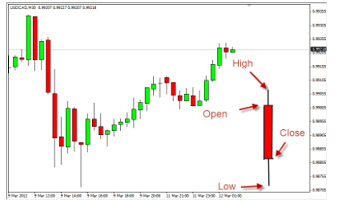
\includegraphics[scale=0.75]{imagenes/candleChart.png}
	\caption{Gráfico de vela.}
\end{figure}

La representación que vamos a adoptar para cada uno de los estados que recibirá el agente, consiste en tomar esta idea de time frame y plasmarla en la estructura de los estados, es decir, el agente será capaz de ver una ventana de tiempo de tamaño n hacia atrás y de diferentes tipos de periodos.

\clearpage

Teniendo en cuenta esto, vamos a definir a cada estado $S_t$  compuesto de 3 capas o layers, de la siguiente forma:
\\\\

$ S_t = L_{dias}, L_{semanas}, L_{meses} \hspace*{1cm} donde \hspace*{0.5cm} L_i = P_1, P_2, ..., P_n $
\\\\
y en donde cada periodo $P_i$ tendrá la siguiente estructura:
\\\\
$P_i$ = Capital\\
\hspace*{0.8cm} Actual Position\\
\hspace*{0.8cm} Open Price\\
\hspace*{0.8cm} Close Price\\
\hspace*{0.8cm} Min Price\\
\hspace*{0.8cm} Max Price\\
\hspace*{0.8cm} Volume\\
\hspace*{0.8cm} ATR\\
\hspace*{0.8cm} MA8\\
\hspace*{0.8cm} EMA20\\
\hspace*{0.8cm} EMA50\\
\hspace*{0.8cm} EMA200\\
\hspace*{0.8cm} RSI\\
\hspace*{0.8cm} DMI\\
\hspace*{0.8cm} MACD\\
\hspace*{0.8cm} BollingerBands\\

\section{Acciones}

En cada instante t el agente podrá decidir comprar, vender o esperar, cada vez que decida comprar o vender, la cantidad de acciones operadas, se calculara en base a una estrategia de entrada y salida del activo pre configurada en el agente.
El agente no tendrá limitación alguna en cuanto a la cantidad de acciones a comprar o vender. Si bien, en la realidad esto no necesariamente seria posible dado que para que pueda comprar una cantidad n a un precio p, debe existir algún vendedor dispuesto a vender n acciones a un precio p cada una.
Ademas cada operación de venta o compra, tendrá un costo asociado c, el cual sera descontado de su capital. El agente no podrá ejecutar la acción elegida si su capital no alcanza para cubrir el costo total de la operación.


\section{El Agente}

Recordemos que el objetivo principal de agente es seleccionar acciones que maximicen su recompensa futura, es decir, deberá de maximizar su capital inicial, para esto vamos a asumir que las recompensa futuras están descontadas por un factor $\gamma$, por cada instante de tiempo t, es decir, vamos a valorizar los rewards más cercanos en el tiempo por un factor $\gamma$. Definimos así el, future discounted reward:
\\\\
\begin{equation}
	 R_t = \sum\limits_{t'= t}^T  \gamma^{t'-t} r_t
\end{equation}

Donde T es el instante en el agente termina de invertir(o bien por qué perdió todo su capital inicial o bien porque se acabaron los datos de simulación).\\
También vamos a definir una función estado-acción óptima, $Q^*(s_t, a_t)$, como la máxima recompensa esperada que podemos alcanzar estando en el estado $s_t$, y seleccionando la acción $a_t$, y luego continuando con una estrategia $\pi$
\\\\
\begin{equation}
Q^*(s, a) = max_{\pi} \E [R_t  |  s_t = s, a_t = a, \pi]
\end{equation}
\\

Esta función tiene una propiedad importante, conocida como Bellman equation, que intuitivamente se basa en lo siguiente: 
Si conociéramos el valor óptimo de $Q^*(s’, a’)$ para el próximo estado s’ y para cada posible acción posible a’, entonces la estrategia óptima de selección de una acción para el estado actual s que maximice la recompensa esperada está dada por
\\\\
\begin{equation}
Q^*(s, a) = max_{\pi} \E_{s' \approx \epsilon} [ r + \gamma max_{a'} Q^*(s', a')  |  s, a]
\end{equation}
\\
La idea general de nuestro algoritmo de aprendizaje va a ser estimar esta función $Q^*$ usando la ecuación de bellman en forma iterativa, esto es:
\\\\
\begin{equation}
Q^*_{i+1}(s, a) = max_{\pi} \E_{s' \approx \epsilon} [ r + \gamma max_{a'} Q_{i}^*(s', a')  |  s, a]
\end{equation}
\\
donde  $i\rightarrow\infty$ y $Q_i \rightarrow Q^*$
\\\\
Esta es la idea detrás del algoritmo de Q-learning que implementará el agente, la cual en principio, parecía suficiente para lograr que el agente aprenda a invertir, sin embargo en la práctica, veremos que en general los estados del mercado no van a repetirse en forma idéntica y que ademas la cantidad de estados posibles hara que sea prácticamente inviable lograr la convergencia hacia $Q^*$.

\section{Q-Network}
Para poder solucionar este inconveniente, vamos a utilizar una función de aproximación, cuyo objetivo será obtener una generalización de los estados, lo cual permitirá en teoría, lograr más rápidamente la convergencia a $Q^*$.\\
Para implementar esta función utilizaremos un red neuronal con con una matriz de pesos $\theta$, inicializada aleatoriamente: 
\\\\
\begin{equation}
Q(s, a, \theta) \approx Q^*(s, a) 
\end{equation}
\\
a la cual denominaremos como Q-network.
Dicha Q-network será entrenada optimizando una función de pérdida L y usando el algoritmo del gradiente descendente.
\\

\begin{equation}
L_i(\theta) = \E_{s, a \approx p(.)}[(y_i - Q(s, a, \theta_i)^2)]
\\\\ 
\end{equation}

\begin{equation}
donde \hspace*{0.5cm}  y_i =  \E_{s \approx \epsilon}[r + \gamma  \hspace*{0.3cm}  max_{a'} Q(s', a', \theta_{i-1}) | s, a]
\end{equation}
\\

Ademas se usara  experience replay para entrenar la Q-Network, es decir, los datos de ejemplos serán generados a partir de la propia experiencia que vaya adquiriendo el agente. Para lograr esto, en cada instante de tiempo t, el agente deberá guardar en un replay memory D, cada experiencia $\epsilon = (s_t, a_t, r_t, s_{t+1})$, observada.
Transcurridos n días el agente deberá ejecutar la fase de entrenamiento de su Q-Network, para esto se generara un mini batch de experiencias pasadas, obtenidas de  su replay memory y con ella se procederá a realizar una última fase actualización de la función de estimación de $Q(s, a, \theta_i)$, usando la regla de actualización de Q-learning y la nueva matriz de pesos $\theta_{i+1}$.


\section{Algoritmo de aprendizaje}

A continuación detallamos el pseudo algoritmo de aprendizaje de nuestro agente.
\\
\\
\begin{algorithm}[1]
\State D $\gets$ new memory\_replay(n)
\State $\theta \gets random() $
\State $Q^*(s, a) \gets Q(\theta)$
\While{$episode \gets generate\_episode() != null$}

\EndWhile
\end{algorithm}


\chapter{Arquitectura y Diseño}

\chapter{Evaluación y Desempeño}


\section{Introducción}

Durante este capitulo nos dedicaremos a analizar el desempeño de nuestro agente. Para ello definiremos una serie de configuraciones, donde haremos variar los diferentes parámetros de ejecución y usaremos cada una de estas configuraciones sobre diferentes compañías para luego tratar de evaluar como dichos parámetros, afectan o no, en el desempeño del mismo. Lo interesante sera observar tanto los patrones de compra y venta ejecutados por el agente durante toda la simulación, como así también las ganancias obtenidas en cada configuración.

\section{Configuraciones}

La siguientes configuraciones serán ejecutas múltiples veces sobre diferente compañías. El objetivo principal de estas configuración es tratar de ver como se comporta el algortimo bajo diferentes seteos. 

En principio hemos considerado 3 configuración que según creemos una sera la  mas optima(moe), una intermedia(lenny) y por ultimo la que peor debería performar sera ralp, pues se acerca mucho a un agente que toma decisiones en forma aleatoria. 

\begin{table}[]
	\centering
	\caption{Configuraciones de los agentes}
	\label{my-label}
	\begin{tabular}{llll}
		Nombre                     & moe & lenny & ralph \\
		$\varepsilon$-greedy       & 0.1 & 0.3   & 1     \\
		learnig rate    $\alpha$   & 0.3 & 0.3   & 0.3   \\
		discount factor $\gamma$   & 0.8 & 0.5   & 0.1   \\
		mini batch                 & 50  & 100   & 5    \\
		memory replay      		   & 500 & 1000  & 10     \\
		hidden layers     		   & 4   & 8     & 2     \\
		neurons per layer  		   & 16  & 32    & 4    
	\end{tabular}
\end{table}

Ambas configuraciones se ejecutaran sobre dos compañías cuyos papeles tienen comportamientos completamente diferentes.
Una apple donde claramente puede verse que el valor de las acciones generalmente se encuentra dentro de un tendencias alcista durante los 10 años y la otra es microsoft la cual posee un comportamiento mas estable, con tramos alcistas, bajistas y tramos donde el papel lateraliza. Las decisiones del agente se mostraran con burbujas de color azul para las compras, y burbujas de color amarillo para las ventas, a media que transcurran los días, se irán marcado cada vela, con una burbuja indicando la acción, para poder simplificar la visualización del gráfico, hemos decidido, no marcar con ningún marcador, los decisiones de esperar.

\section{Resultados}

\subsection{moe}
Estos son algunos de los resultados de la primera ejecución de moe sobre ambas compañías.

\begin{figure}[h!]
	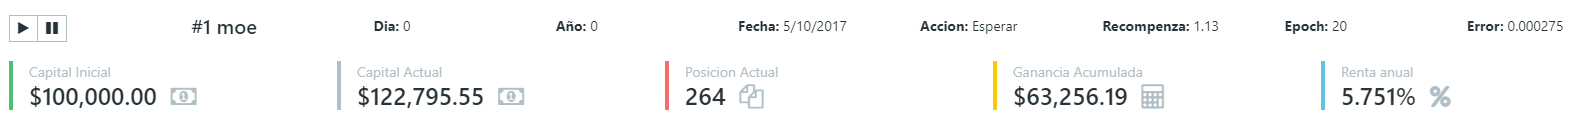
\includegraphics[scale=0.5]{imagenes/moe_appl_ex1_1_summary.png}
	\caption{Resultados de moe sobre apple}
\end{figure}

\begin{figure}[h!]
	
\includegraphics[scale=0.45]{imagenes/moe_msft_ex1_1_summary.png}
	\caption{Resultados de moe sobre microsoft}
\end{figure}

En este caso, el agente logro mejores resultados con apple, probablemente producto de la propia característica de un papel generalmente alcista.
Sin embargo, observemos que sucede durante los primeros días de la simulación.

\begin{figure}[h!]
	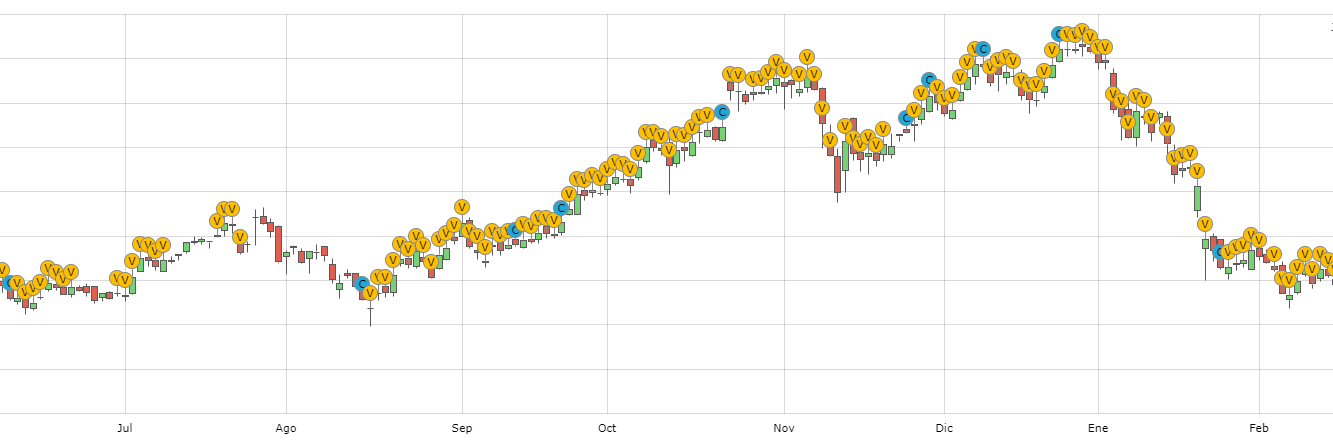
\includegraphics[scale=0.5]{imagenes/moe_appl_ex1_1.png}
	\caption{Primeros días de trading sobre apple}
\end{figure}

\begin{figure}[h!]
	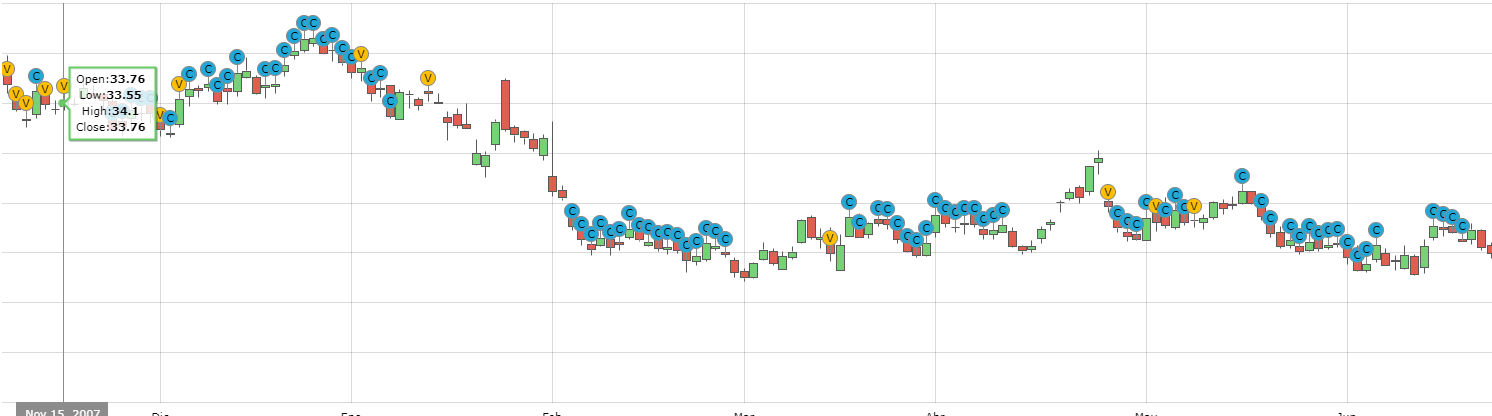
\includegraphics[scale=0.45]{imagenes/moe_msft_ex1_1.png}
	\caption{Primeros días de trading sobre microsoft}
\end{figure}

Claramente puede observarse que el agente se predispone mayoritariamente a realizar siempre la misma acción, en el primer caso decide vender, y en el segundo comprar.
Probablemente esto este determinado por la elección de la primera acción, pues sera la que en principio mas se repita, y de la que mayor conocimiento tiene sobre su recompenza futura. A media que vaya experimentado en forma aleatoria otras acciones, gracias a la policy $\varepsilon$-greedy, deberiamos esperar ver un cambio en el patrón de decisiones.
Veamos ahora que sucede con los últimos días de trading:

\begin{figure}[h!]
	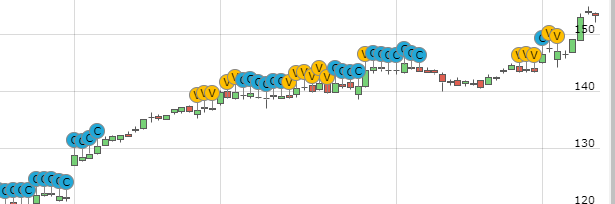
\includegraphics[scale=0.7]{imagenes/moe_appl_ex1_2.png}
	\caption{Últimos días de trading sobre apple}
\end{figure}

\begin{figure}[h!]
	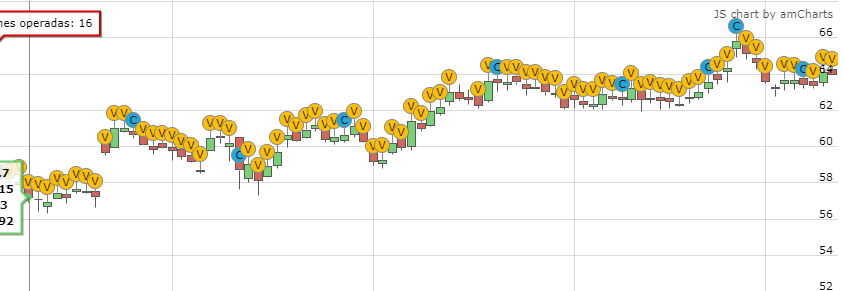
\includegraphics[scale=0.7]{imagenes/moe_msft_ex1_2.png}
	\caption{Últimos días de trading sobre microsoft}
\end{figure}

En ambos casos, puede observarse una mejoría, tal vez, en el caso de apple sea mas marcada, dado que hasta puede observarse que durante varios días, el agente solo decide esperar, y especular esperando que el precio suba para vender luego de varios días gran parte de sus acciones a un precio mucho mayor al que las compro.
Para el caso de microsoft, no es tan claro, pero sin embargo, puede verse que cada 4 o  5 días, el agente compra, para luego vender. Es importante notar aquí, que dado el esquema de entrada y salida que se decidió adoptar, los días en que compra, comprar mucho mas de lo que luego vende en los días siguientes.

Un aspecto interesante que surgió durante la investigación, fe preguntarnos que sucedería si volviéramos a ejecutar el agente ya entrado, es decir, reutilizando la matriz de pesos de su red neuronal.
¿Podría el agente mejorar su performance?.

Estos son los resultados que obtuvimos para moe

\begin{figure}[h!]
	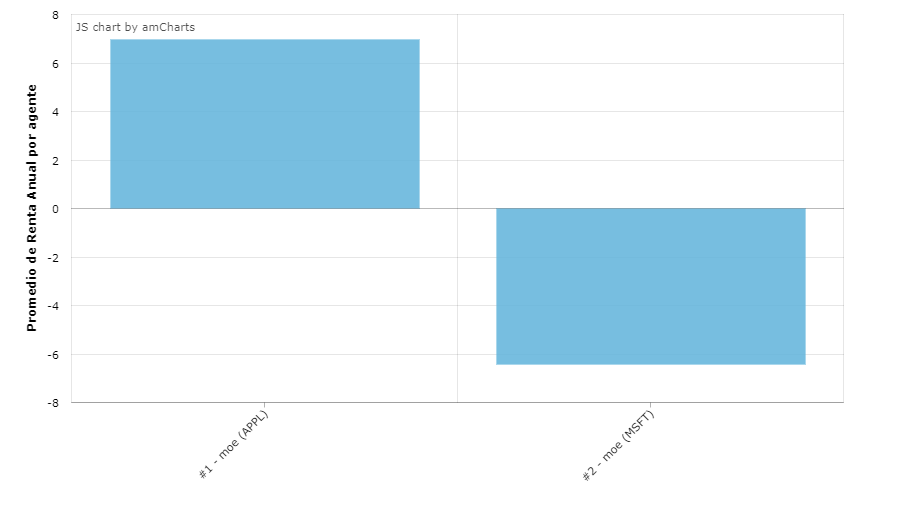
\includegraphics[scale=0.7]{imagenes/moe_results_1.png}
	\caption{Promedio del rate de ganancias finales}
\end{figure}

\begin{figure}[h!]
	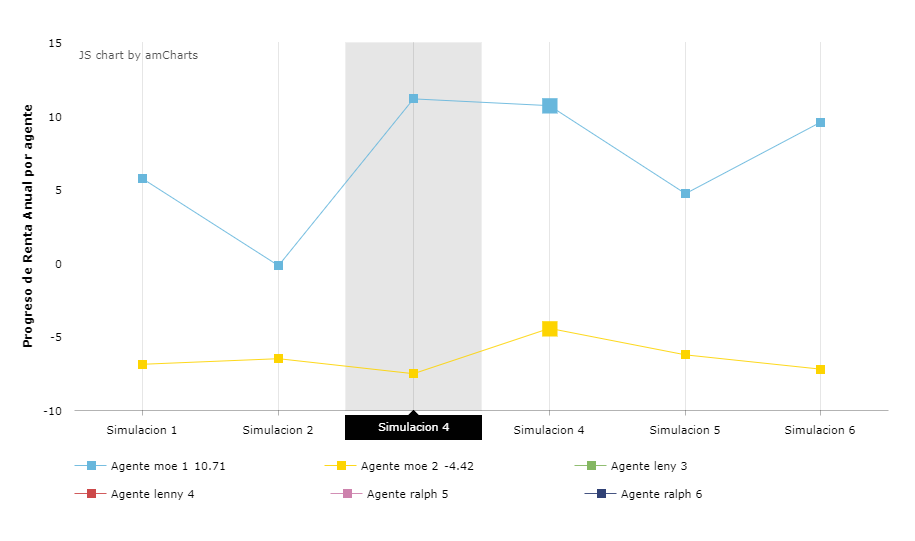
\includegraphics[scale=0.7]{imagenes/moe_results_2.png}
	\caption{Evolución de ganancias}
\end{figure}

Mirando los gráficos resultantes, no pareciera a ver una mejoría significativa, aunque si podemos afirmar que los agentes en general, repitieron su performance. Sin embargo pudimos observar una notoria modificación en el patrón de decisiones del agente:

\begin{figure}[h!]
	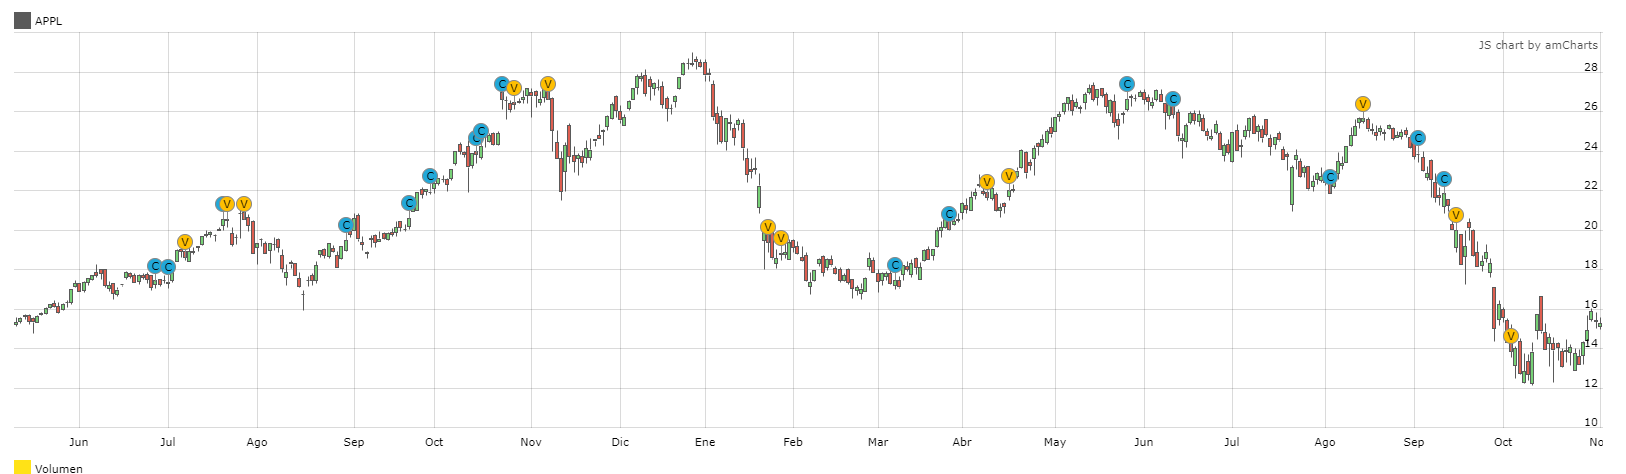
\includegraphics[scale=0.4]{imagenes/moe_appl_ex6_1.png}
	\caption{Resultados de moe luego de 6 ejecuciones}
\end{figure}

Claramente podemos notar, que el agente toma decisiones de compra y/o venta mucho mas espaciadas en el tiempo, a comparación de las primeras ejecuciones, donde el agente tendía a sobre operar en el mercado, y terminaba realizado compras y ventas diariamente. No podemos concluir si esto significa una mejora o no, aunque si es posible asociar este tipo de patrón a un comportamiento mucho mas especulativo.

\subsection{lenny}

Como podíamos esperar, efectivamente lenny, se desempeño peor que moe.
Sin embargo también podemos observar un cambio en el patrón de desicion a lo largo del tiempo.

\begin{figure}[h!]
	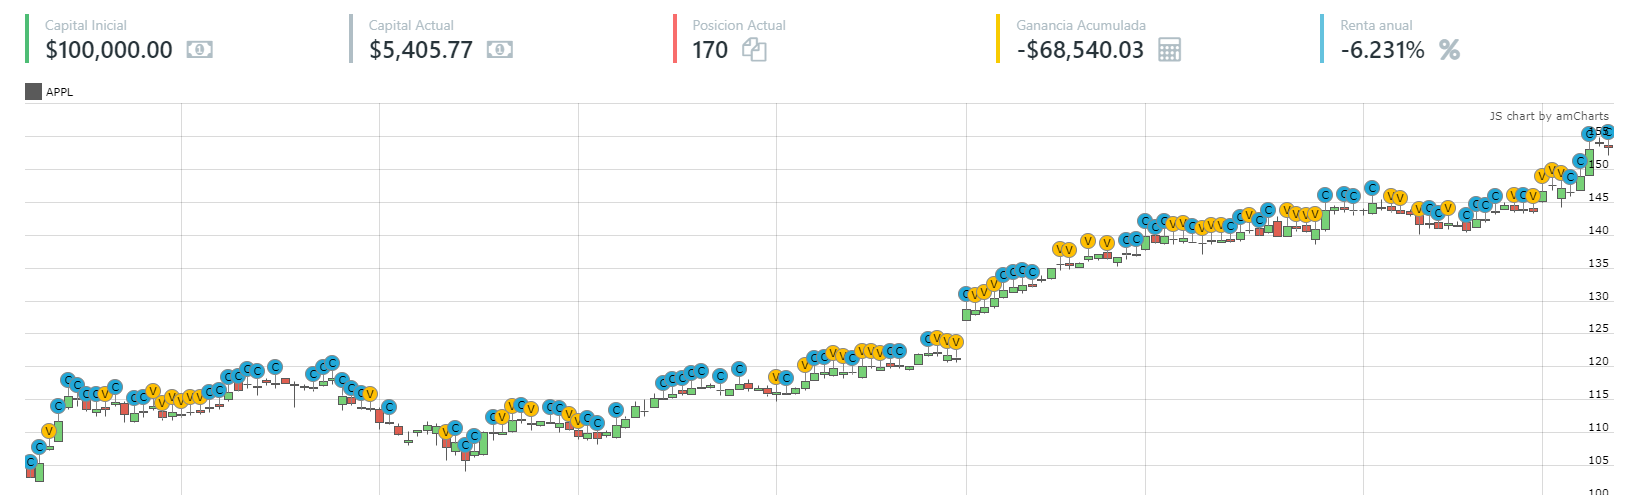
\includegraphics[scale=0.5]{imagenes/lenny_appl_ex1_1.png}
	\caption{Ejecución de lenny sobre apple}
\end{figure}

\begin{figure}[h!]
	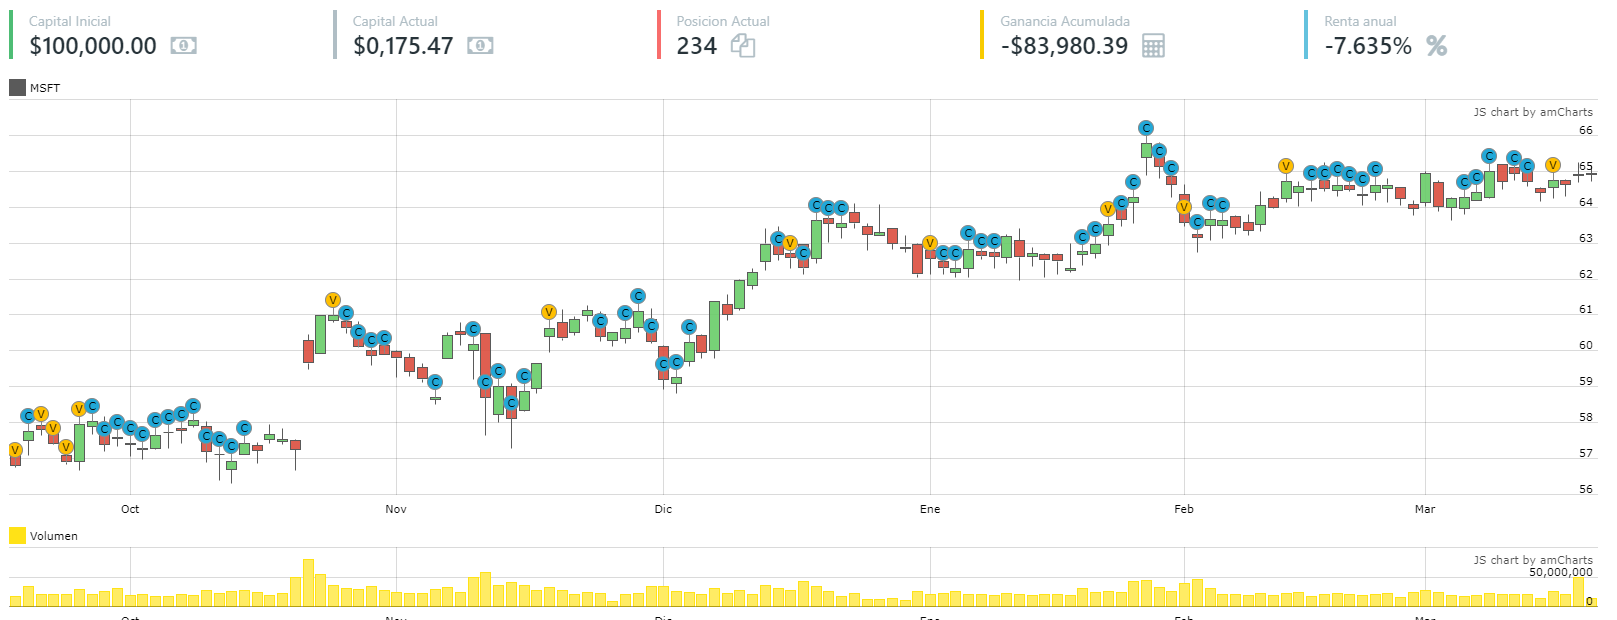
\includegraphics[scale=0.5]{imagenes/lenny_msft_ex1_1.png}
	\caption{Ejecución de lenny sobre microsoft}
\end{figure}


\subsection{ralph}
Por ultimo, nos que analizar con ralp, y nuevamente, se dio lo que esperamos, si bien los resultados en términos del rate de ganancias, no difieren tanto, si podemos observa que el patrón de decisiones del agente se mantiene en el tiempo, dado que efectivamente siempre elige aleatoriamente. También pudimos observar un error muy grande durante el entrenamiento de la QNetwork, y que en general, dicho error no se reduce, provocando la no convergencia de la función Q

\begin{figure}[h!]
	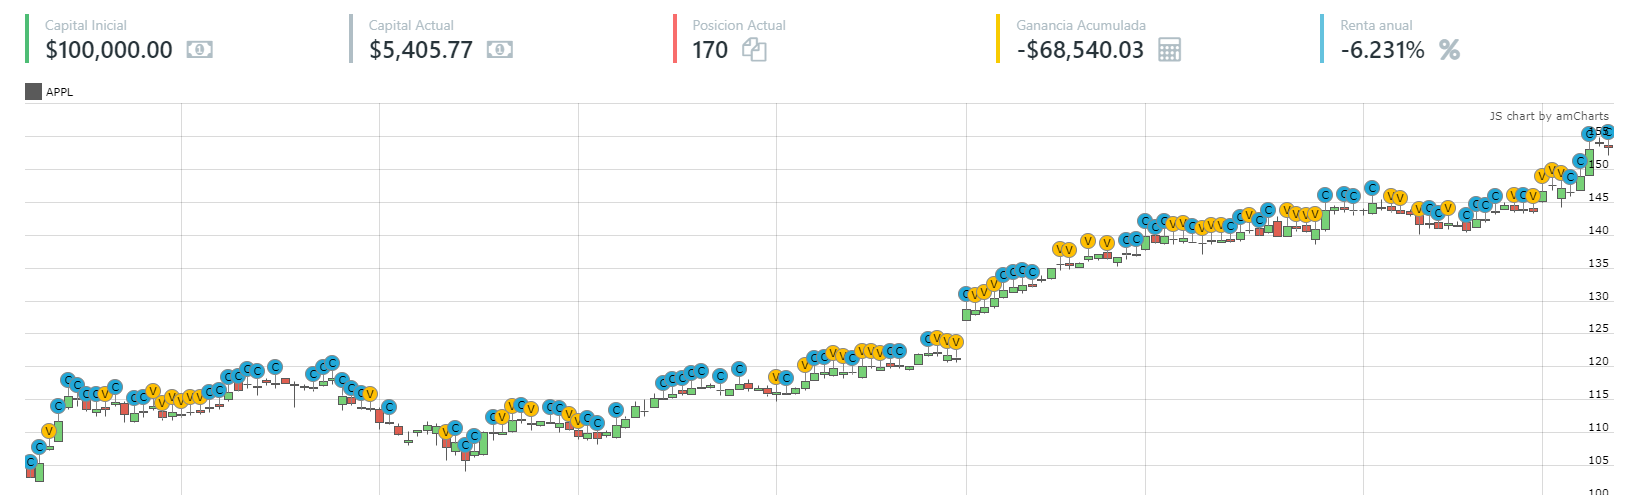
\includegraphics[scale=0.4]{imagenes/lenny_appl_ex1_1.png}
	\caption{Ejecución de ralph sobre apple}
\end{figure}

\begin{figure}[h!]
	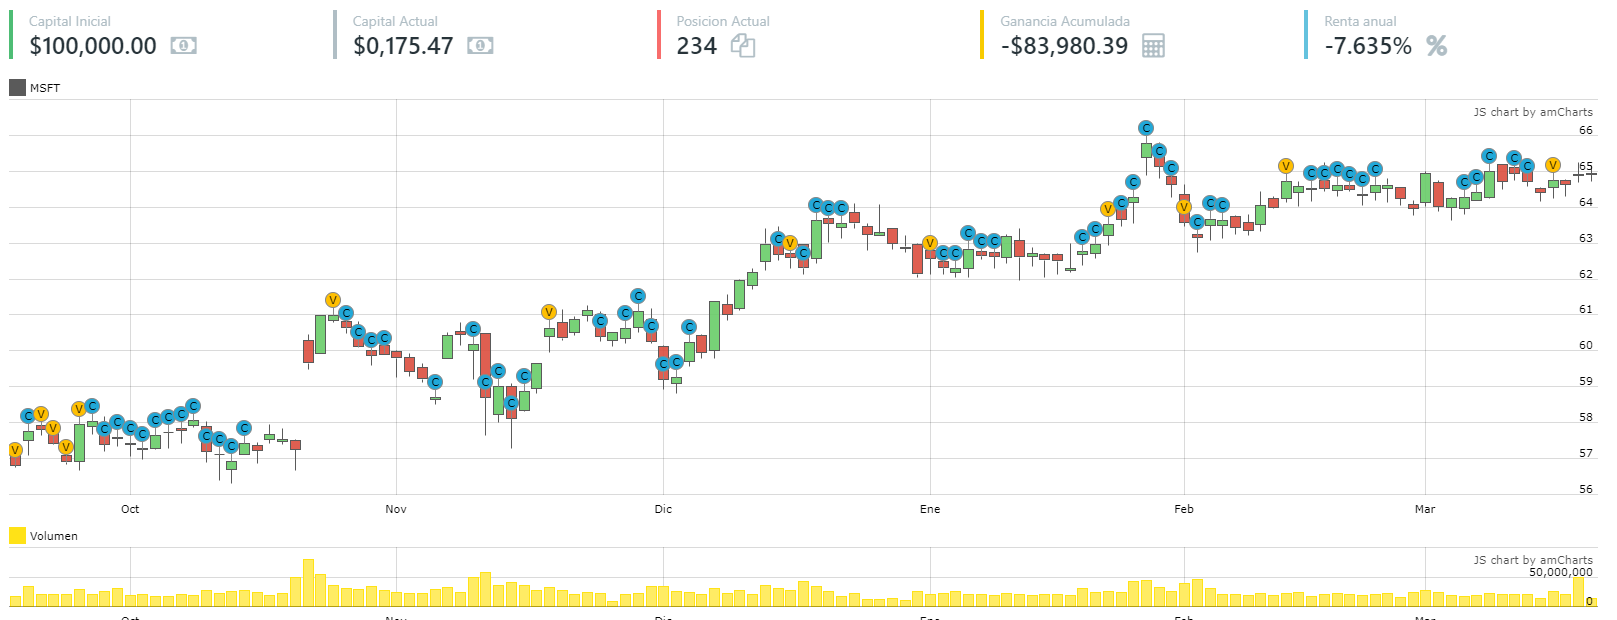
\includegraphics[scale=0.4]{imagenes/lenny_msft_ex1_1.png}
	\caption{Ejecución de ralph sobre microsoft}
\end{figure}

\section{Gráficos}


\chapter{Conclusiones}

Durante este capitulo final, queremos comentar algunas observaciones y/o recomendaciones que creemos es necesario resaltar.
Recordemos que el objetivo inicial del proyecto era investigar la posible aplicabilidad y efectividad del uso de reinforcement learning y deep learning en el desarrollo de sistemas de trading. Luego de varios días de desarrollo y pruebas, y que mas allá de los resultados obtenidos, que tal vez estén lejos de igualar o sustituir a un inversor experimentado, el sistema demostró ser fiable en el sentido de es posible implementar un algoritmo que solamente evaluando la evolución del precio de un activo, aprenda a tomar decisiones sobre el.\\ Podemos no estar conforme con las ganancias obtenidas, pero es claro que es posible generar un proceso de aprendizaje, el cual le permite al agente mejorar su desempeño a lo largo del tiempo, como así también poder repetirlo en simulaciones siguientes.
\\\\
También, debemos reconocer aquí nuestra falta de experiencia y comprensión en el diseño y desarrollo de redes neuronales, el cual es posible que haya podido influenciar en la performance del agente. O que tal vez, el uso de una red neuronal no sea la mejor solución para estimar la función de valor $Q(s, a)$, en cualquier caso, creemos que el potencial de mejora en este aspecto es enorme, y que junto con ello, la posibilidad de mejorar el desempeño de nuestro a agente.\\

Por otro lado, queremos resaltar, que no nos resulto sencillo determinar la efectividad de la performance del agente, es decir, no fue sencillo determinar cuando un trade es bueno o no, y en particular poder determinar si una decisión de compra o venta, es correcta o no. Tal vez también, producto de nuestra falta de conocimiento y/o entendimiento de los mercados.Y por lo tanto, también, en este sentido, creemos que hay mucha posibilidad de mejoras, y con ello poder modificar la señal de recompensa para tratar de mejorar el proceso de aprendizaje del agente.\\

En definitiva, podemos decir que los resultados son prometedores, y que como prueba de concepto ha logrado satisfacer nuestras expectativas, lo que nos permite pensar que en un futuro no muy lejano, este tipo de sistemas sean mas comunes ya sea como soporte a inversores o como sistemas completamente automatizados que permitan la administración de una cartera de inversiones.
\chapter{Bibliografía}


\begin{itemize}	
	\item \href{http://people.inf.elte.hu/lorincz/Files/RL_2006/SuttonBook.pdf}{\textcolor{blue}{Reinforcement Learning: An Introduction - Richard S. Sutton and Andrew G. Barto.}}
	\item \href{http://rll.berkeley.edu/deeprlcourse/}{\textcolor{blue}{Bekerly UC - Curse: Deep Reinforcement Learning}}
	\item \href{http://karpathy.github.io/2016/05/31/rl/}{\textcolor{blue}{Stanford - Curse: Convolutional Neural Networks for Visual Recognition}}
	\item \href{http://neuralnetworksanddeeplearning.com/}{\textcolor{blue}{Neural Networks and Deep Learning}}
	\item \href{http://www.doc.ic.ac.uk/teaching/distinguished-projects/2015/j.cumming.pdf}{\textcolor{blue}{An Investigation into the Use of Reinforcement Learning Techniques within the Algorithmic Trading Domain}}
	\item \href{http://cs229.stanford.edu/proj2009/LvDuZhai.pdf}{\textcolor{blue}{Algorithm Trading using Q-Learning and Recurrent Reinforcement Learning}}
	\item \href{http://neuro.cs.ut.ee/demystifying-deep-reinforcement-learning/}{\textcolor{blue}{Demystifying deep reinforcement learning}}
	\item \href{https://arxiv.org/pdf/1312.5602v1.pdf}{\textcolor{blue}{Original DeepMind paper}}
	\item Stock Price prediction using  reinforcement learning - Jae Won Lee - June 2001
	\item Reinforcement learning for optimized trade execution - Yuriy Nevmayvaka, Yi Feng, Micheal Kearns - June 2006
	\item Reinforcement learning and savings behavior - James J. Choi, David Laibson, Brigitte C. Madrian, Andrew Metrick - November 2009
	\item Continuous control with deep reinforcement learning, Timothy P. Lillicrap, Jonathan J. Hunt, Alexander Pritzel, Nicolas Heess, Tom Erez, Yuval Tassa, David Silver, Daan Wierstra - 2016
\end{itemize}
\bibliography{eieclases_ref}

\clearpage

%------------------
\end{document}
